\documentclass[11pt, a4paper]{article}
\usepackage{pdfpages}
\usepackage{parallel}
\usepackage[T2A]{fontenc}
\usepackage{ucs}
\usepackage[utf8x]{inputenc}
\usepackage[polish,english,russian]{babel}
\usepackage{hyperref}
\usepackage{rotating}
\usepackage[inner=2cm,top=1.8cm,outer=2cm,bottom=2.3cm,nohead]{geometry}
\usepackage{listings}
\usepackage{graphicx}
\usepackage{wrapfig}
\usepackage{longtable}
\usepackage{indentfirst}
\usepackage{array}
\usepackage{tikzsymbols}
\usepackage{soul}
\usepackage[ruled,vlined]{algorithm2e}
%\counterwithout{figure}{section} 

\usepackage{url}
\makeatletter
\g@addto@macro{\UrlBreaks}{\UrlOrds}
\makeatother

\newcolumntype{P}[1]{>{\raggedright\arraybackslash}p{#1}}
\frenchspacing
\usepackage{fixltx2e} %text sub- and superscripts
\usepackage{icomma} % коскі ў матэматычным рэжыме
\PreloadUnicodePage{4}

\newcommand{\longpage}{\enlargethispage{\baselineskip}}
\newcommand{\shortpage}{\enlargethispage{-\baselineskip}}

\def\switchlang#1{\expandafter\csname switchlang#1\endcsname}
\def\switchlangbe{
\let\saverefname=\refname%
\def\refname{Літаратура}%
\def\figurename{Іл.}%
}
\def\switchlangen{
\let\saverefname=\refname%
\def\refname{References}%
\def\figurename{Fig.}%
}
\def\switchlangru{
\let\saverefname=\refname%
\let\savefigurename=\figurename%
\def\refname{Литература}%
\def\figurename{Рис.}%
}

\hyphenation{admi-ni-stra-tive}
\hyphenation{ex-pe-ri-ence}
\hyphenation{fle-xi-bi-li-ty}
\hyphenation{Py-thon}
\hyphenation{ma-the-ma-ti-cal}
\hyphenation{re-ported}
\hyphenation{imp-le-menta-tions}
\hyphenation{pro-vides}
\hyphenation{en-gi-neering}
\hyphenation{com-pa-ti-bi-li-ty}
\hyphenation{im-pos-sible}
\hyphenation{desk-top}
\hyphenation{elec-tro-nic}
\hyphenation{com-pa-ny}
\hyphenation{de-ve-lop-ment}
\hyphenation{de-ve-loping}
\hyphenation{de-ve-lop}
\hyphenation{da-ta-ba-se}
\hyphenation{plat-forms}
\hyphenation{or-ga-ni-za-tion}
\hyphenation{pro-gramming}
\hyphenation{in-stru-ments}
\hyphenation{Li-nux}
\hyphenation{sour-ce}
\hyphenation{en-vi-ron-ment}
\hyphenation{Te-le-pathy}
\hyphenation{Li-nux-ov-ka}
\hyphenation{Open-BSD}
\hyphenation{Free-BSD}
\hyphenation{men-ti-on-ed}
\hyphenation{app-li-ca-tion}

\def\progref!#1!{\texttt{#1}}
\renewcommand{\arraystretch}{2} %Іначай формулы ў матрыцы зліпаюцца з лініямі
\usepackage{array}

\def\interview #1 (#2), #3, #4, #5\par{

\section[#1, #3, #4]{#1 -- #3, #4}
\def\qname{LVEE}
\def\aname{#1}
\def\q ##1\par{{\noindent \bf \qname: ##1 }\par}
\def\a{{\noindent \bf \aname: } \def\qname{L}\def\aname{#2}}
}

\def\interview* #1 (#2), #3, #4, #5\par{

\section*{#1\\{\small\rm #3, #4. #5}}
\ifx\ParallelWhichBox\undefined%
    \addcontentsline{toc}{section}{#1, #3, #4}%
\else%
\ifnum\ParallelWhichBox=0%
    \addcontentsline{toc}{section}{#1, #3, #4}%
\fi\fi%

\def\qname{LVEE}
\def\aname{#1}
\def\q ##1\par{{\noindent \bf \qname: ##1 }\par}
\def\a{{\noindent \bf \aname: } \def\qname{L}\def\aname{#2}}
}

\newcommand{\interviewfooter}[1]{
\vskip 1em
\noindent \textit{#1}
}

\switchlang{ru}
\begin{document}

\title{1982 "--- Hawley Mark II X063X Mouse}
\date{}
\maketitle
\selectlanguage{russian}
Мышь Mark II X063X Mouse (рис. \ref{fig:HawleyMarkIIPic}) стала первой собственной разработкой компании Hawley Mouse House \cite{hawley,mouses}, созданной Джеком Хоули, соразработчиком мыши для компьютеров Xerox Alto и одним из авторов патента Xerox 1973 года на мышь с двумя наклонными колесами \cite{pat}. Цена мыши в \$415 \cite{buxton} вдохновила обозревателей назвать ее <<Роллс-Ройсом среди мышей>>.

\begin{figure}[h]
   \centering
    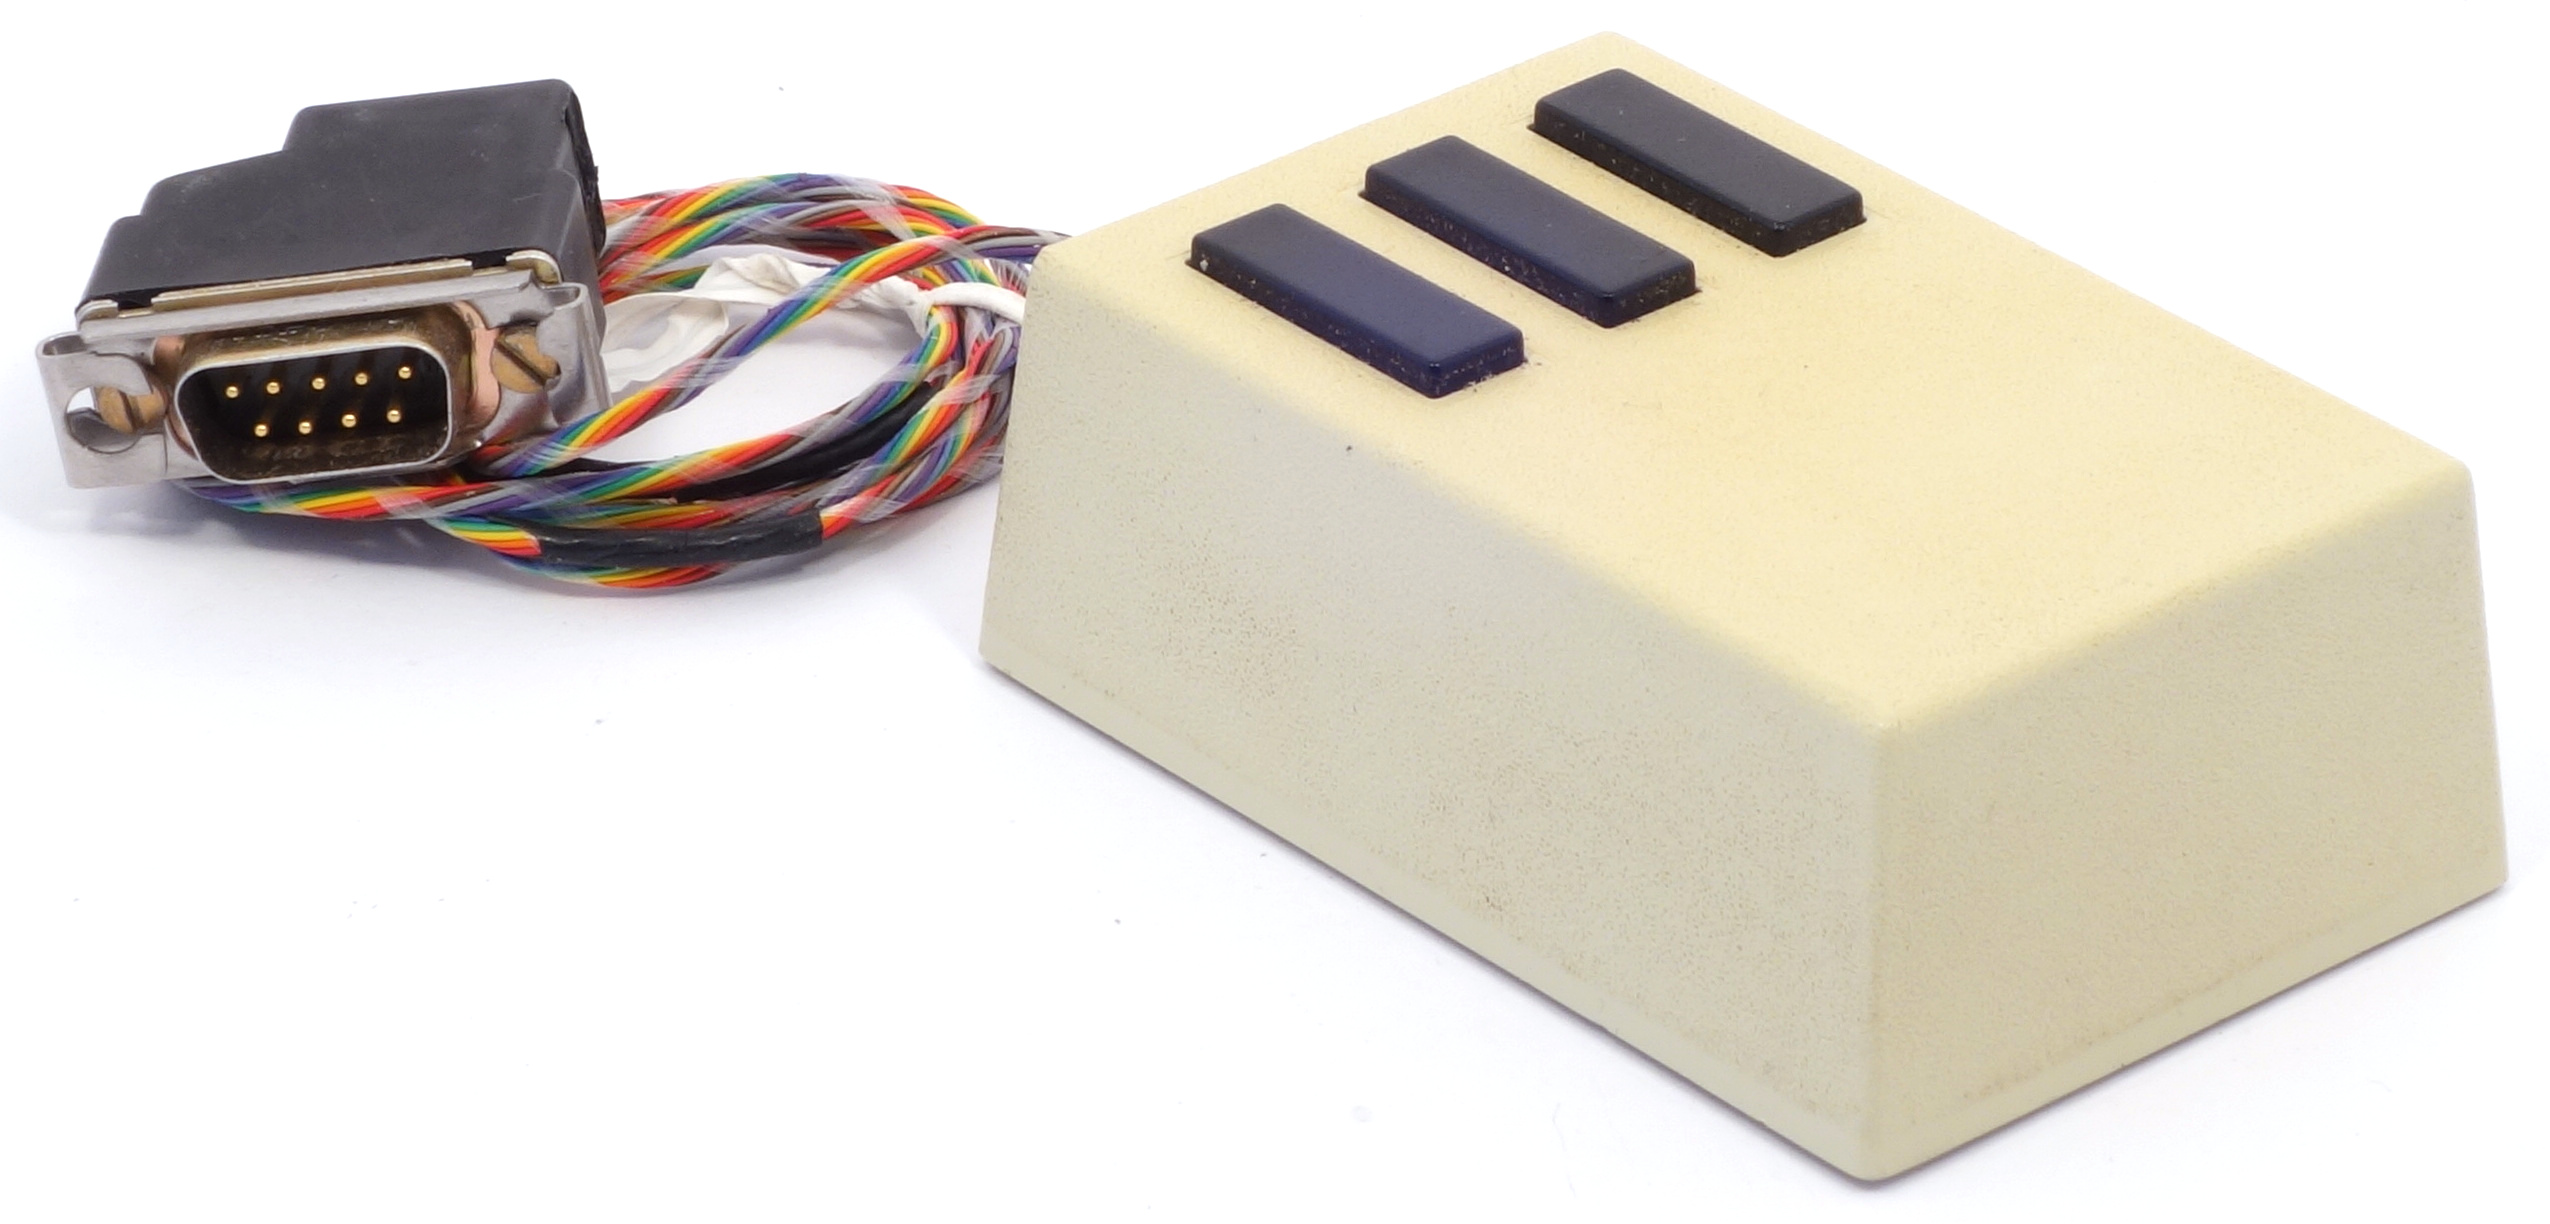
\includegraphics[scale=0.6]{1982_hawley_mark_ii/pic_60.jpg}
    \caption{Hawley Mark II X063X Mouse, вид спереди}
    \label{fig:HawleyMarkIIPic}
\end{figure}

Мышь Mark II X063X выполнена в доведенном до крайней степени индустриальном дизайне: корпус представляет собой почти правильный паралеллепипед, на котором расположены три прямоугольные кнопки цвета, максимально контрастного по отношению к корпусу (рис. \ref{fig:HawleyMarkIITopAndBottom}). Очевидно, дизайн был призван подчеркнуть целевое назначение мыши, ориентированной на инженеров и пользователей различных САПР (включая твердотельное моделирование и архитектуру).

Данный экземпляр является бежевым с черными кнопками (на кабеле можно заметить остатки черной изоляции, утратившей со временем эластичность и рассыпавшейся на части). Распространенным также был вариант с противоположным сочетанием цветов корпуса и кнопок, а также известно еще несколько вариантов расцветки. Реклама Hawley дает представление о возможных сочетаниях цветов \cite{brochure}, однако нет информации о том, сколько вариантов расцветки из этой рекламной фотографии было реализовано на практике.

\begin{figure}[h]
    \centering
    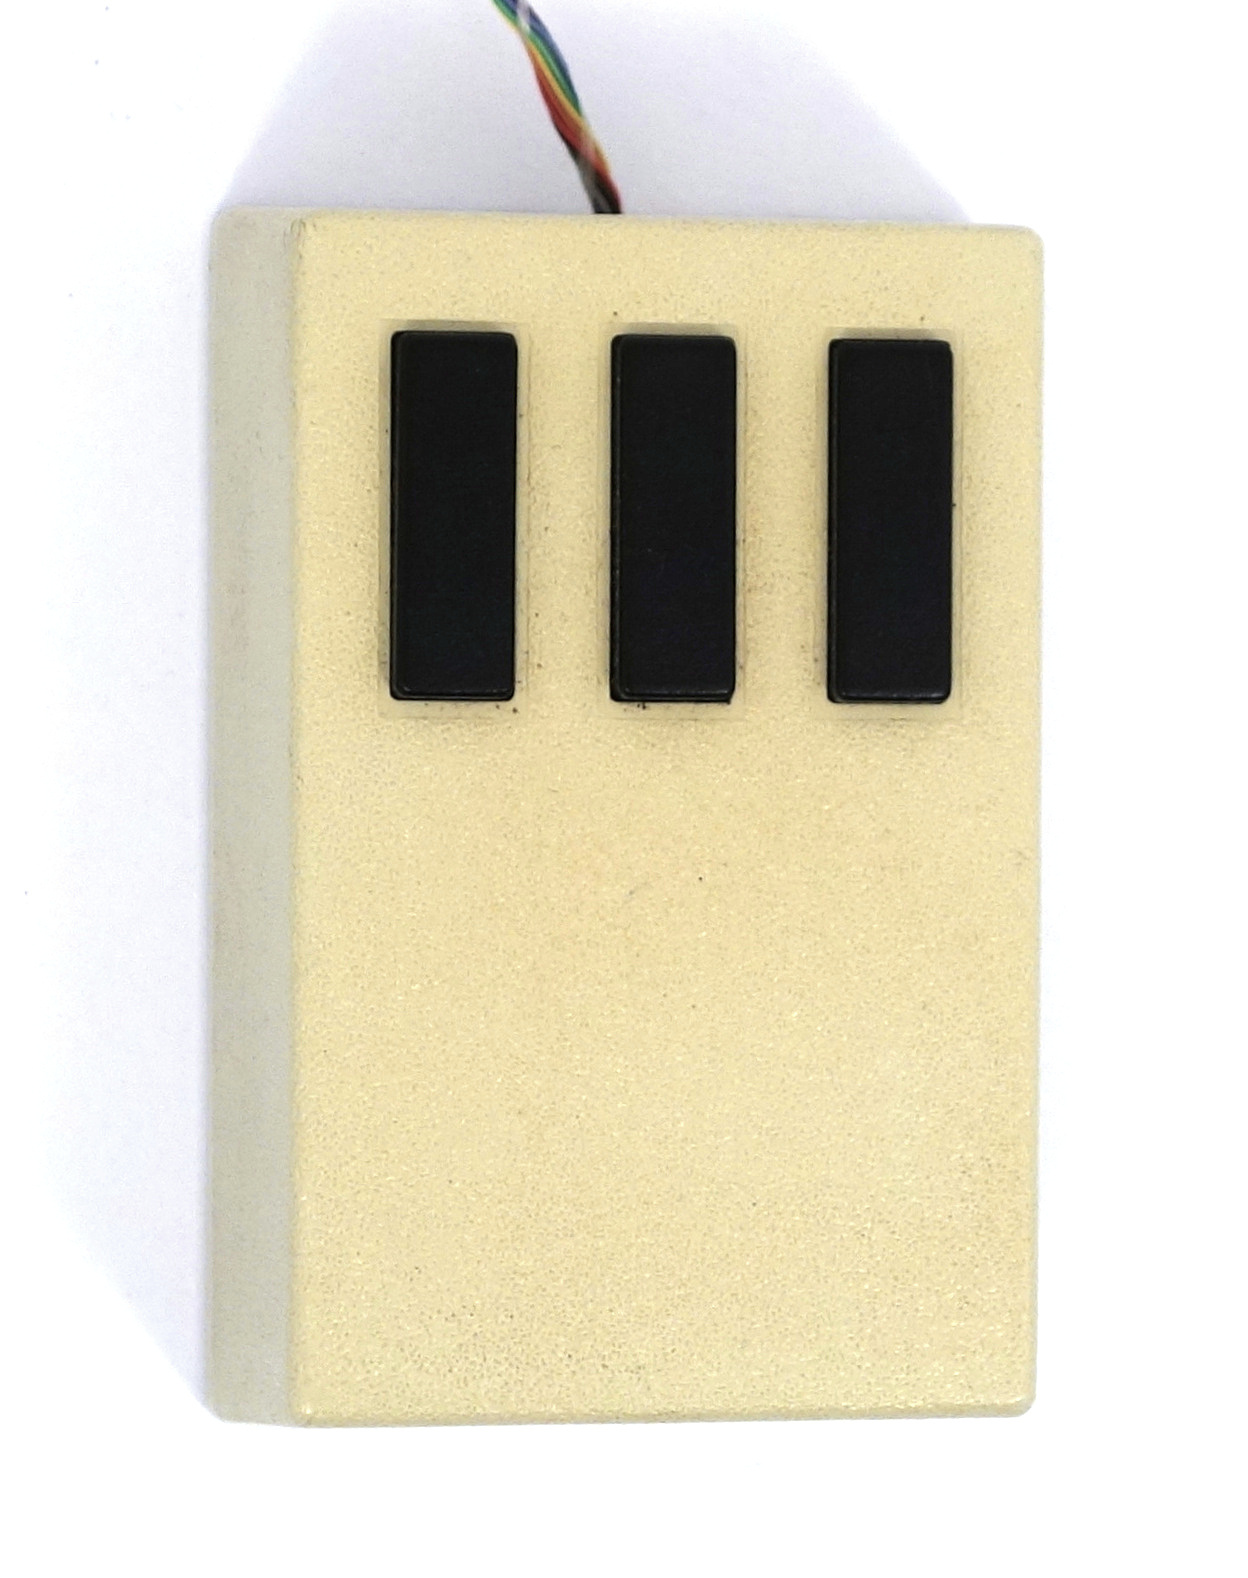
\includegraphics[scale=0.45]{1982_hawley_mark_ii/top_60.jpg}
    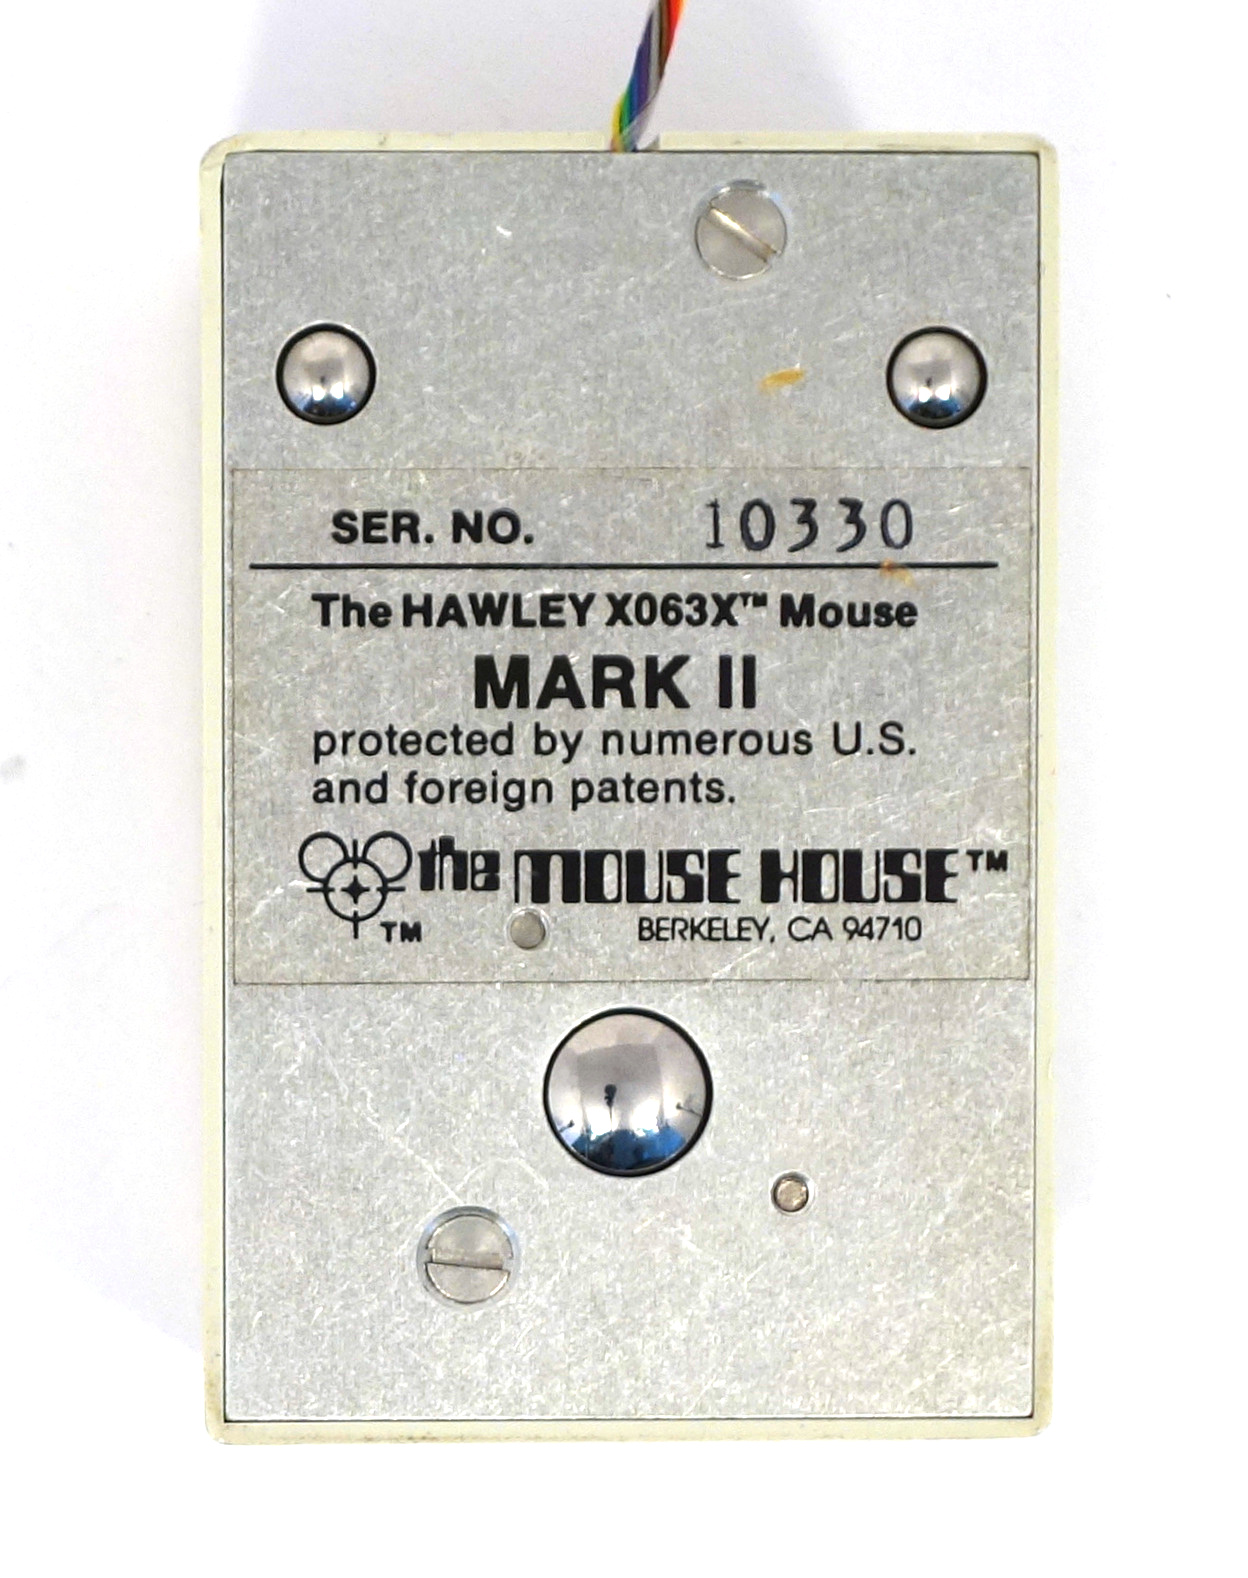
\includegraphics[scale=0.45]{1982_hawley_mark_ii/bottom_60.jpg}
    \caption{Hawley Mark II X063X Mouse, вид сверху и снизу}
    \label{fig:HawleyMarkIITopAndBottom}
\end{figure}



Нижняя стоорона целиком выполнена из металла (рис. \ref{fig:HawleyMarkIITopAndBottom}). Вращение регистрируется гладким стальным шаром в центре, а еще два шарика меньшего размера играют роль ножек для минимизации трения. Съемное кольцо, позволяющее извлечь шар для удаления собравшегося мусора, в данной модели еще не предусмотрено, поэтому для чистки необходима полная разборка.

\begin{figure}[h]
    \centering
    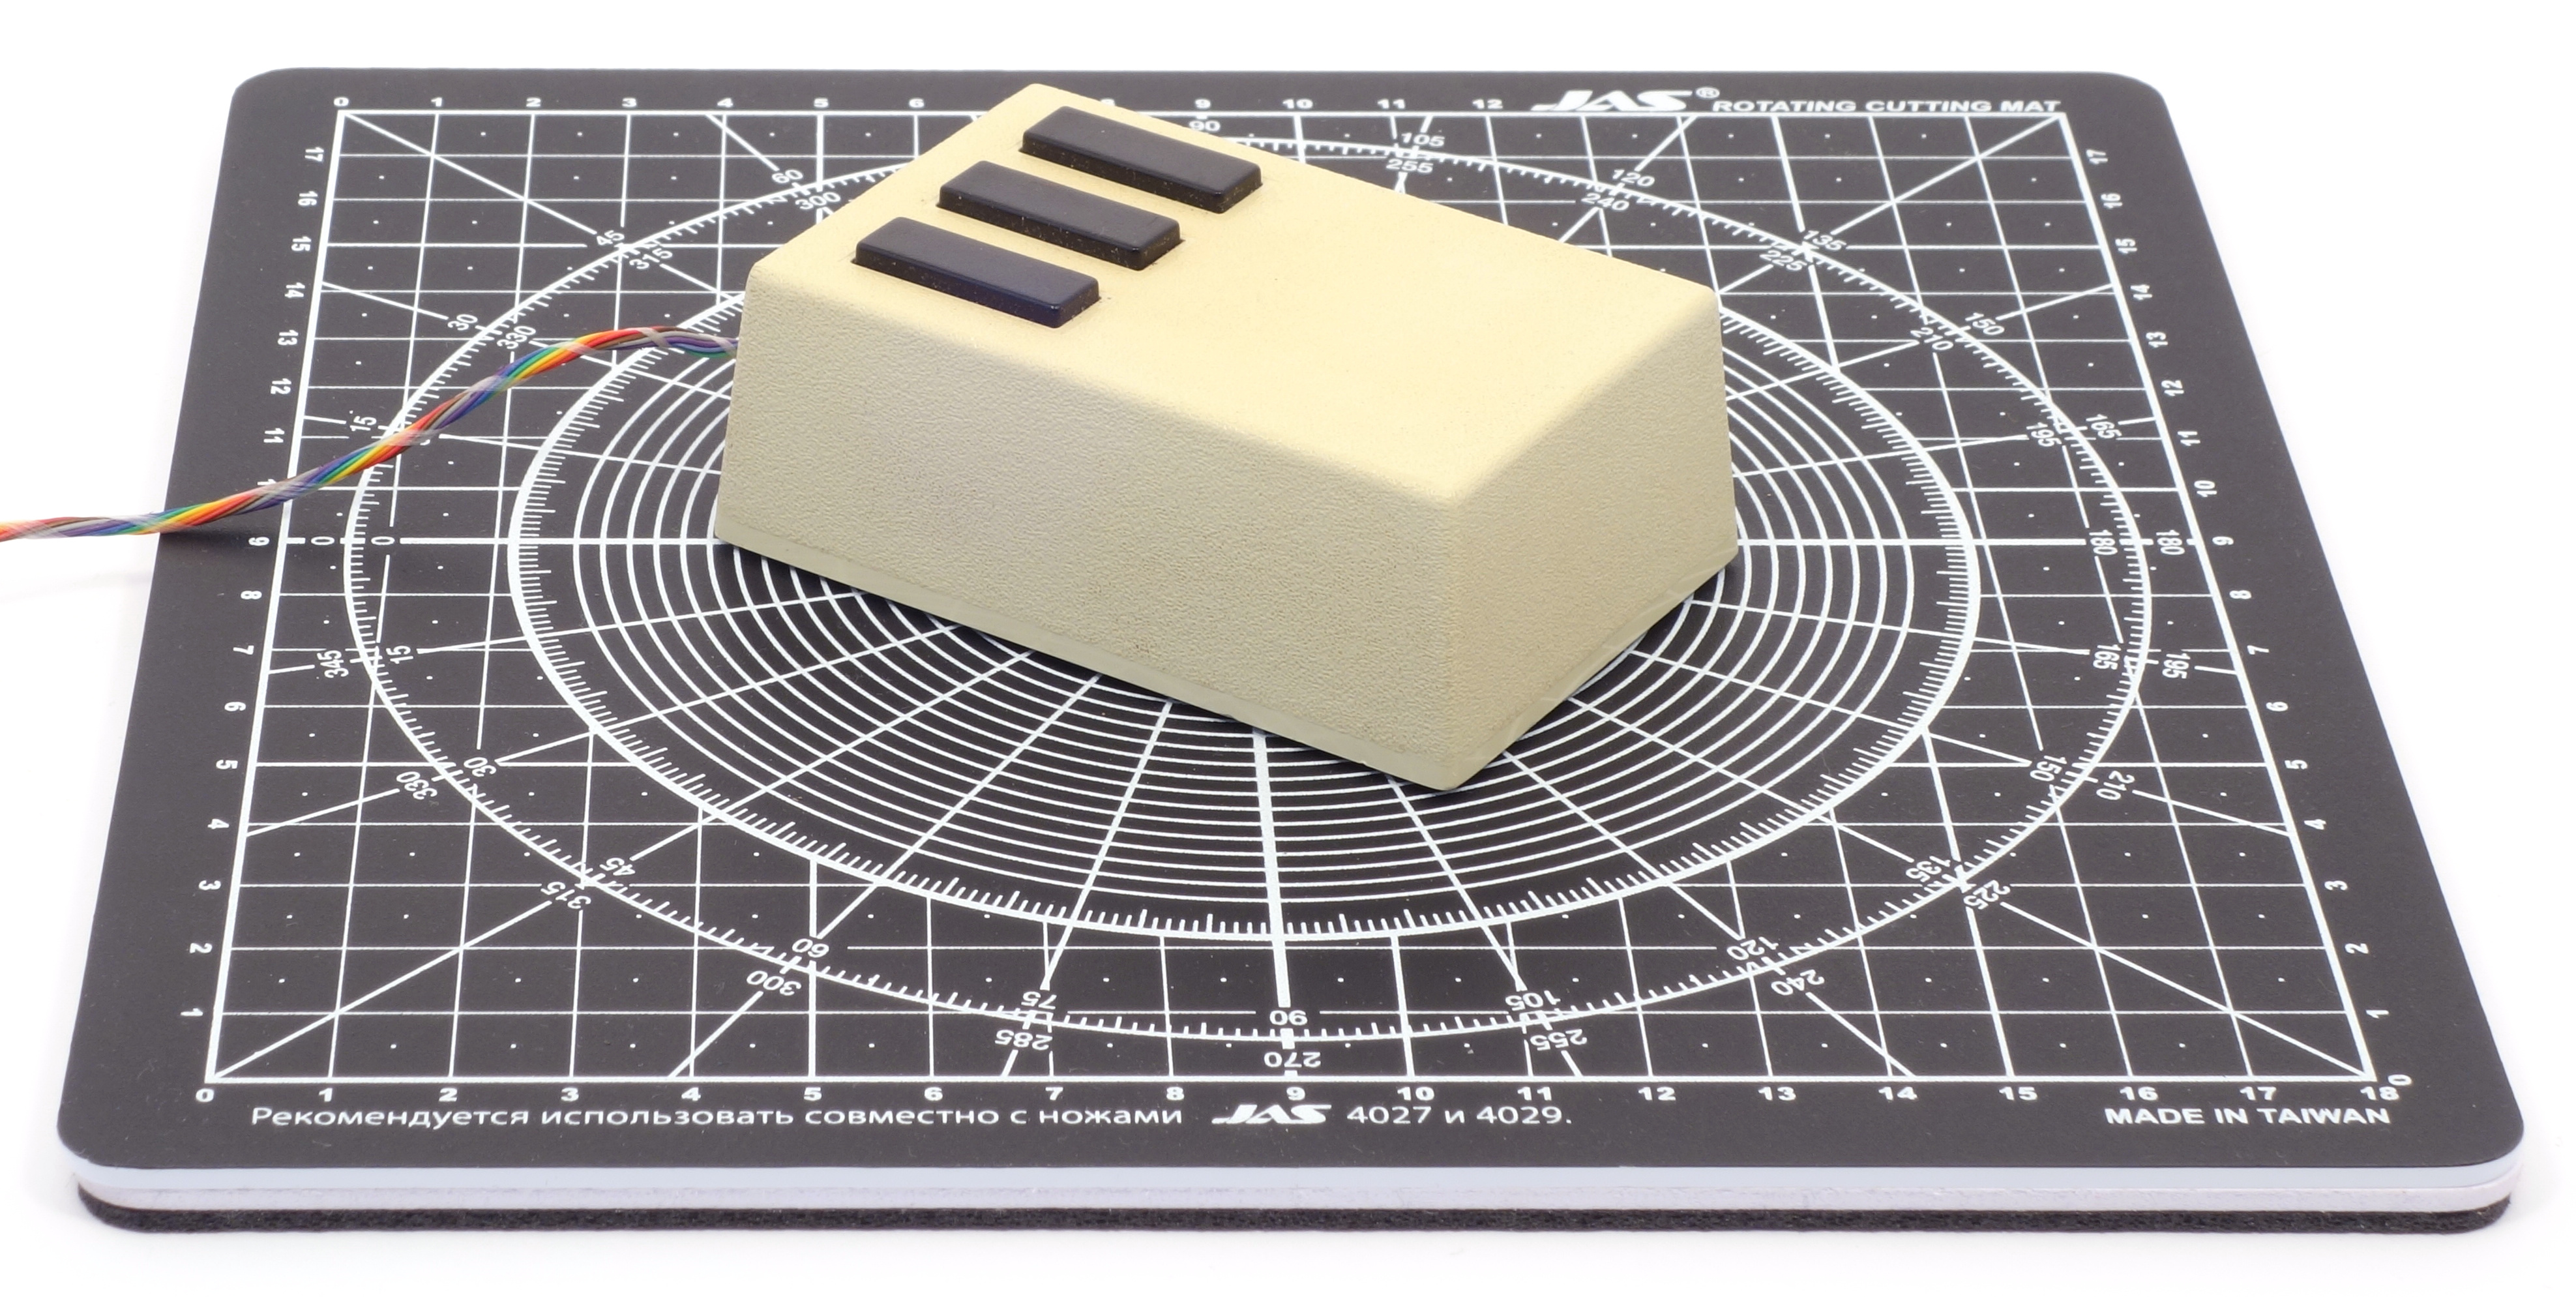
\includegraphics[scale=0.5]{1982_hawley_mark_ii/size_30.jpg}
    \caption{Hawley Mark II на размерном коврике с шагом сетки 1~см}
    \label{fig:HawleyMarkIISize}
\end{figure}

Мышь имеет небольшие размеры, характерные для мышей 1980-х годов (рис. \ref{fig:HawleyMarkIISize}). Очевидно, это хотя бы немного уменьшает негативное влияние корпуса с ортогональными гранями на эргономику, поскольку рука может опереться на корпус лишь в незначительной степени (рис. \ref{fig:HawleyMarkIIHand}).

\begin{figure}[h]
    \centering
    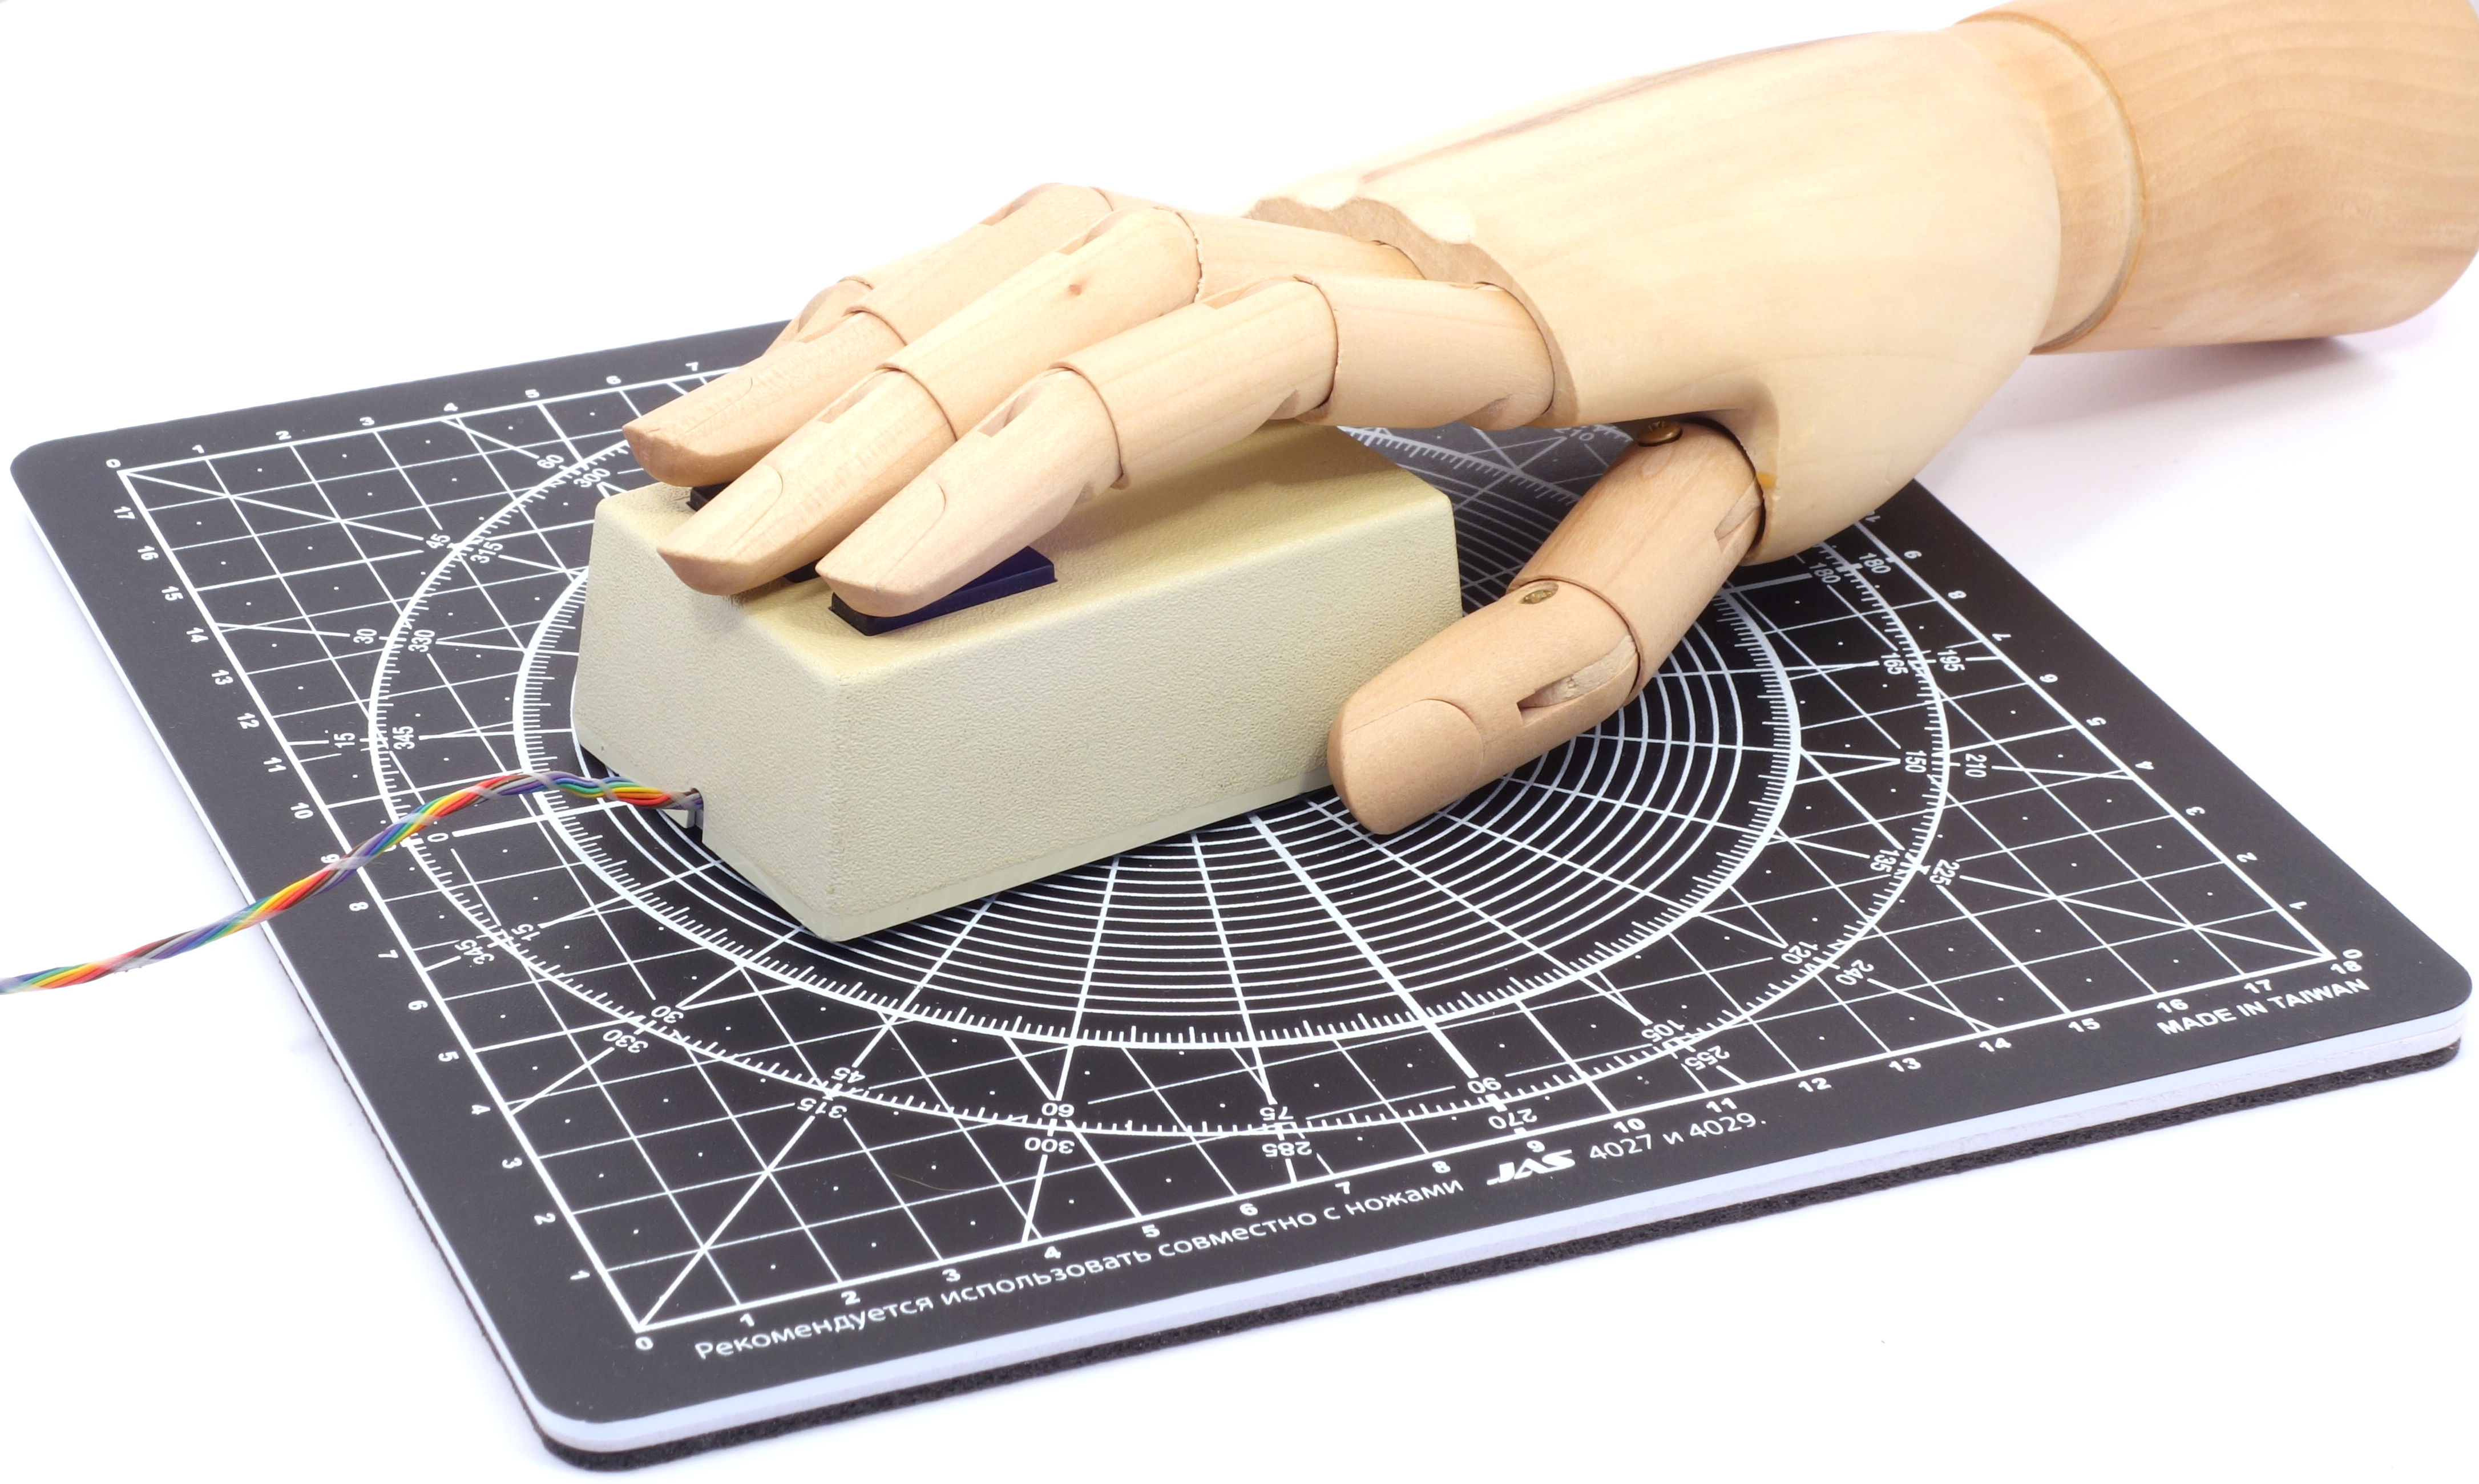
\includegraphics[scale=0.5]{1982_hawley_mark_ii/hand_60.jpg}
    \caption{Hawley Mark II с моделью руки человека}
    \label{fig:HawleyMarkIIHand}
\end{figure}

Внутреннее устройство мыши показано на рис. \ref{fig:HawleyMarkIIInside}. Можно отметить съемную глухую защиту шара, требующую дополнительных операций разборки для удаления мусора. В мыши испольованы механические энкодеры, представляющие собой металлический контактный барабан (вместо более распространенного в более поздних моделях диска) и четыре контакта различной длины вместо двух для увеличения разрешающей способности энкодера.

 \begin{figure}[h]
    \centering
    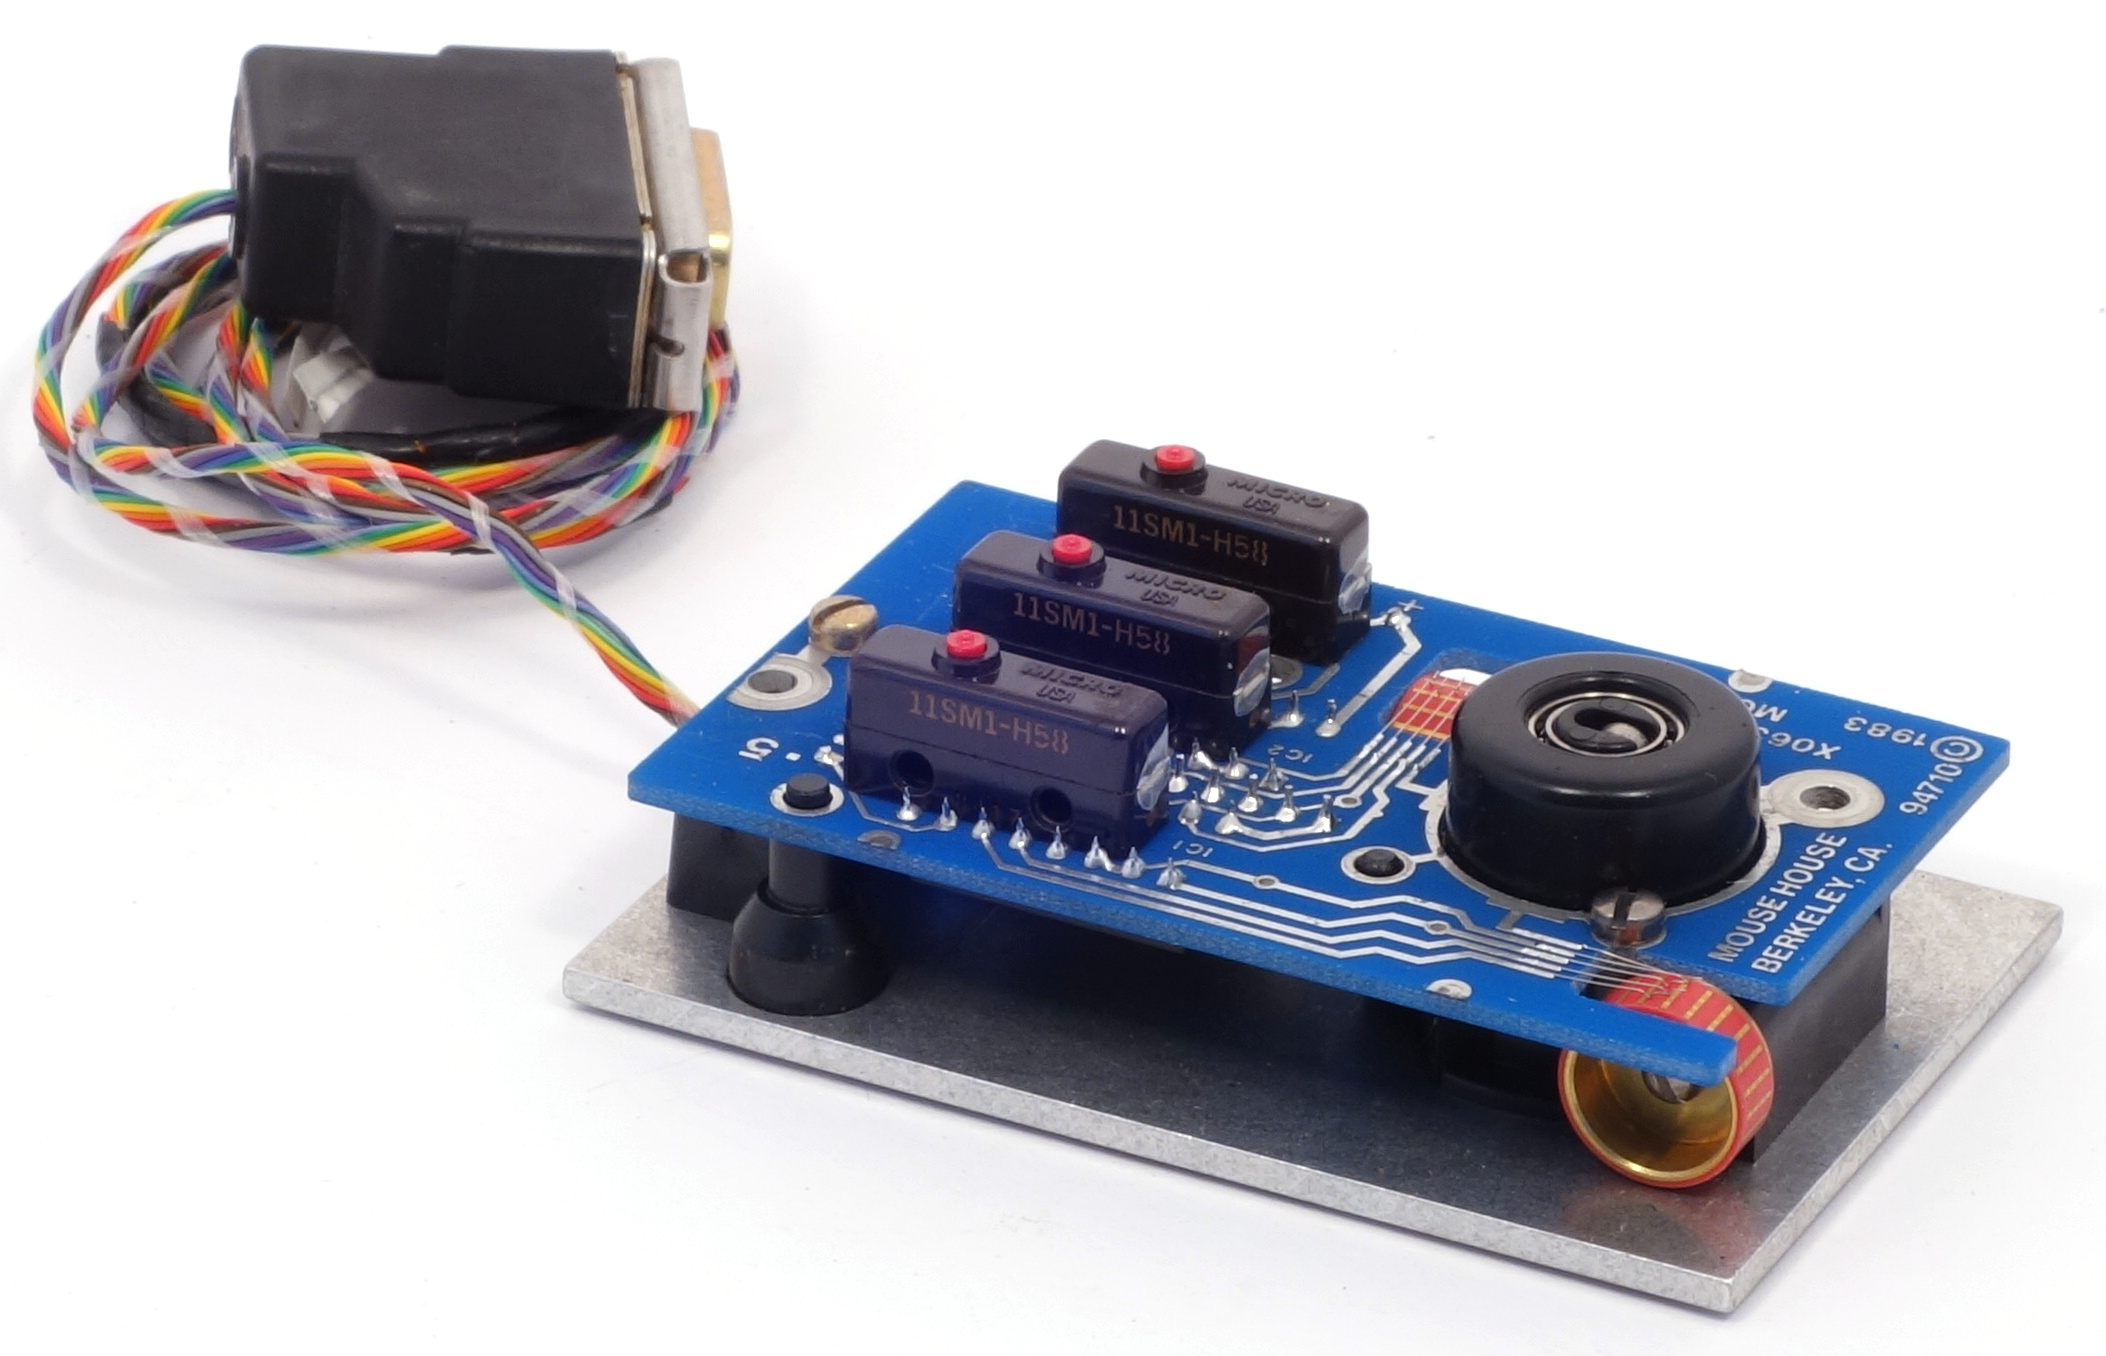
\includegraphics[scale=0.8]{1982_hawley_mark_ii/inside_60.jpg}
    \caption{Hawley Mark II в разобранном виде}
    \label{fig:HawleyMarkIIInside}
\end{figure}

\begin{thebibliography}{9}
\bibitem{hawley} Hawley Mouse House \url{https://web.archive.org/web/20211020150835/https://oldmouse.com/mouse/hawley/}
\bibitem{mouses} Hawley Mark II X063X Mouses \url{https://web.archive.org/web/20211020000256/https://www.oldmouse.com/mouse/hawley/X063X.shtml}
\bibitem{pat} Transducer for a display-oriented pointing device \url{https://patents.google.com/patent/US3892963A/en}
\bibitem{buxton} Buxton collection. Hawley Mouse MK II \url{https://www.microsoft.com/buxtoncollection/detail.aspx?id=141}
\bibitem{brochure} Mouse House MK II Brochure \url{https://www.microsoft.com/buxtoncollection/a/pdf/Mouse%20House%20MK%20II%20Brochure.pdf}
\end{thebibliography}
\end{document}
